\documentclass[tikz]{standalone}

\usepackage{fontspec}
\usepackage{mathtools}
\usepackage{unicode-math}
\usepackage{siunitx}

\newcommand{\az}{\ensuremath{\Phi}}
\newcommand{\el}{\ensuremath{\theta}}

% Tikz Style
\usepackage{tikz}

\usetikzlibrary{decorations.markings}
\usetikzlibrary{arrows.meta}

\usepackage{pgfplots}
\pgfplotsset{
  compat=1.18
  ,width=15cm
  ,lua debug
}

\definecolor{celestial}{rgb}{1,0,1}%{0.0, 0.51, 0.5}
\definecolor{elevation}{rgb}{0,1,0}%{0.6, 0.4, 0.8}
\definecolor{horizon}{rgb}{0,0,1}%{0.54, 0.81, 0.94}
\definecolor{sun}{rgb}{0.83, 0.0, 0.25}

\tikzstyle{help circle} = [dashed, thick]
\tikzstyle{coordinate curve} = [ultra thick]
\tikzstyle{sun position} = [color=sun,ultra thick]
\tikzstyle{navi direction} = [font=\sffamily\Large]
\tikzstyle{coordinate angle} = [font=\Large]
\tikzstyle{base plane} = [font=\sffamily]

\begin{document}
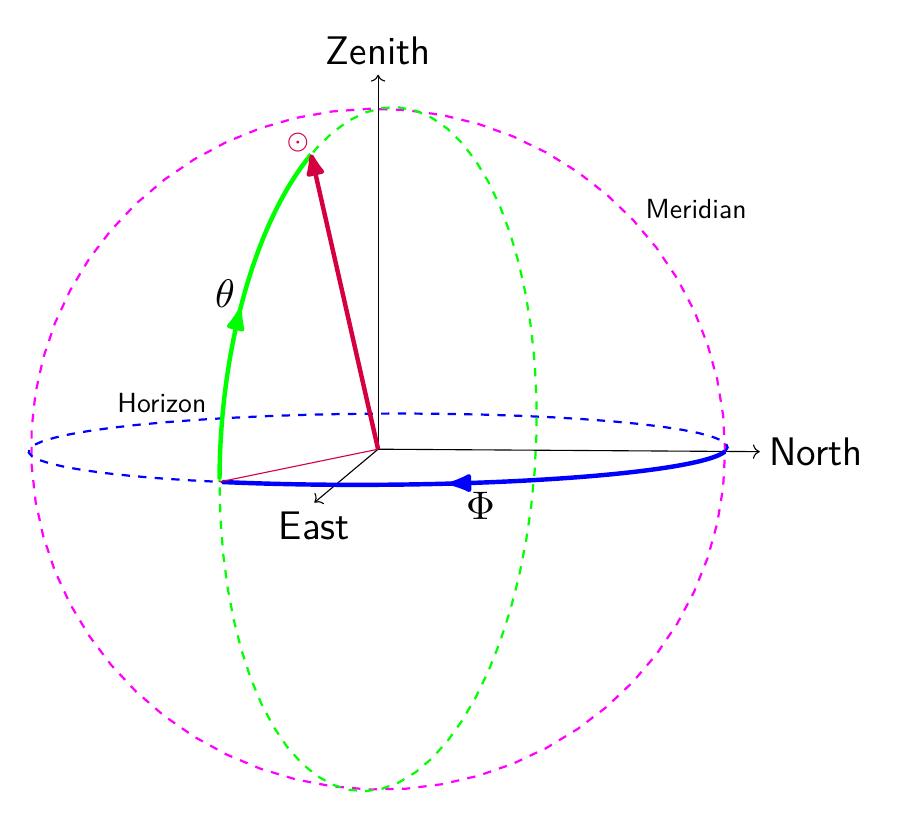
\begin{tikzpicture}
\begin{axis}[view={5}{5}
  ,axis lines=none,
  ,plot box ratio={1 1 1}
  ,xlabel=$x$
  ,ylabel=$y$
  ,zlabel=$z$
  ,xmin=-1.4
  ,xmax=1.4
%  ,ymin=-1.2
%  ,ymax=1.2
%  ,zmin=-1.2
%  ,zmax=1.2
  ,declare function={
% Sun position
  azimuth=-110;  % Positive = westward from north
  elevation = 65; % Positive = from Horizon to Zenith
  sunx = cos(azimuth)*cos(elevation);
  suny = sin(azimuth)*cos(elevation);
  sunz = sin(elevation);
% Text Az coordinates
  textazx = cos(3/5*azimuth);
  textazy = sin(3/5*azimuth);
  textazz = 0;
% Text El coordinates
  textelx = cos(azimuth)*cos(elevation/2);
  textely = sin(azimuth)*cos(elevation/2);
  textelz = sin(elevation/2);
% Celestial Meridian
    ucx = 1;
    ucy = 0;
    ucz = 0;
%
    vcx = 0;
    vcy = 0;
    vcz = 1;
    celestialx(\t) = cos(\t)*ucx + sin(\t)*vcx;
    celestialy(\t) = cos(\t)*ucy + sin(\t)*vcy;
    celestialz(\t) = cos(\t)*ucz + sin(\t)*vcz;
% Horizon => Azimut
    uhx = 1;
    uhy = 0;
    uhz = 0;
%
    vhx = 0;
    vhy = 1;
    vhz = 0;
    horizonx(\t) = cos(\t)*uhx + sin(\t)*vhx;
    horizony(\t) = cos(\t)*uhy + sin(\t)*vhy;
    horizonz(\t) = cos(\t)*uhz + sin(\t)*vhz;
% Elevation
    uex = cos(azimuth);
    uey = sin(azimuth);
    uez = 0;
%
    vex = 0;
    vey = 0;
    vez = 1;
    elevationx(\t) = cos(\t)*uex + sin(\t)*vex;
    elevationy(\t) = cos(\t)*uey + sin(\t)*vey;
    elevationz(\t) = cos(\t)*uez + sin(\t)*vez;
  }
]
%
\draw[->] (0,0,0) -- (1.1,0,0) node[anchor=west,navi direction]   {North};
\draw[->] (0,0,0) -- (0,-1.5,0) node[anchor=north,navi direction] {East};
\draw[->] (0,0,0) -- (0,0,1.1) node[anchor=south,navi direction]  {Zenith};
\node at ( 0.71,    0,0.71)[anchor=west,outer sep=1ex,base plane] {Meridian}; %0.71 app sqrt(2)/2
\node at (-0.71, 0.71,0)   [anchor=south,base plane]              {Horizon};
% Plot the Meridian through Nord
\addplot3 [
  domain=0:360,
  samples=60,
  samples y=1,
  variable=t,
  celestial,help circle
] (
 {celestialx(t)},
 {celestialy(t)},
 {celestialz(t)}
);
% Plot the horizon circle
\addplot3 [
  domain=0:360,
  samples=60,
  samples y=1,
  variable=t,
  horizon,help circle
] (
 {horizonx(t)},
 {horizony(t)},
 {horizonz(t)}
);
% Plot the azimuth curve
\addplot3 [
  domain=0:azimuth+0.5,
  samples=60,
  samples y=1,
  variable=t,
  horizon,coordinate curve,
  postaction={decorate},
  decoration={markings,
    mark=at position 0.55 with {\arrow{Latex[round]}}
  }
] (
 {horizonx(t)},
 {horizony(t)},
 {horizonz(t)}
);
% Plot the great circle through the sun
\addplot3 [
  domain=0:360,
  samples=60,
  samples y=1,
  variable=t,
  elevation,help circle
] (
 {elevationx(t)},
 {elevationy(t)},
 {elevationz(t)}
);
% Plot the elevation curve
\addplot3 [
  domain=0.5:elevation,
  samples=60,
  samples y=1,
  variable=t,
  elevation,coordinate curve,
  postaction={decorate},
  decoration={markings,
    mark=at position 0.5 with {\arrow{Latex[round]}}
  }
] (
 {elevationx(t)},
 {elevationy(t)},
 {elevationz(t)}
) ;
\draw [-{Latex[round]}, sun position] (0,0,0) -- (sunx, suny, sunz) node[anchor=south east,inner sep=0] {$\odot$};
\draw [sun position, thin](0,0,0) -- (uex, uey, 0);
\node at (textazx, textazy, textazz) [anchor=north,coordinate angle] {\az};
\node at (textelx, textely, textelz) [anchor=east ,coordinate angle] {\el};
\end{axis}
\end{tikzpicture}

\end{document}


